\chapter{Описание алгоритма}
\label{cha:ch_2}

\section{Теоретическое обоснование алгоритма}

\textbf{Энергия от частоты}, нужно умножить амплитуду на $f$.
Отметим также, что \textbf{}

\begin{figure}
  \centering
  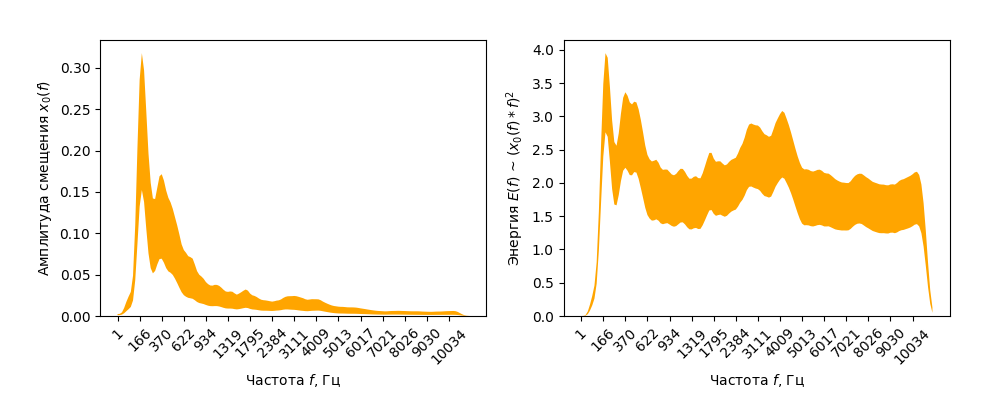
\includegraphics[width=0.9\linewidth]{figures/spectrum_mean}
  \caption{Распределение амплитуды и энергии по частоте. Энергия пропорциональна квадрату амплитуды скорости}
  \label{fig:spectrum_mean}
\end{figure}

\begin{markdown}
 - Оконное фурье через свертку
   - метод, окна, частоты, неопределенность
   - вычислительная сложность
 - оптимальный размер окна для конкретной шкалы частот
 - оптимальная форма окна для устойчивости к искажениям
 - Восстановление сигнала через свертку
 - Критерий восстановимости
 - восстановление сигнала с наложением
 - шкала амплитуд
 - выбор оптимальной шкалы частот
   - мел шкала
   - линейная шкала
   - комбинированная шкала
 - рекомендуемые значения параметров
 - связь количества частот и разрешения по времени
 - точность восстановления
 - избыточность информации в шумах
 - представление с сохранением фазы
 - представление с производной фазы
 - представление с магнитудой
 - Алгоритм Гриффина-Лима
  - адаптация
  - более точное восстановление при сохранении фазы
 - картинки
\end{markdown}

\section{Реализация алгоритма}
\begin{markdown}
 - описание алгоритма
   - подготовка ядра
     - шкала частот, df
	 - окна для каждой частоты
	 - Фурье базис с окнами, нормировка
	 - маска наложений
	 - ядро прямого прохода
	 - ядро обратного прохода
   - прямое преобразование
     - свертка
	 - преобразование фазы
	   - либо ничего
	   - либо производная фазы
	   - либо только магнитуда
	 - шкала амплитуд
   - обратное преобразование
     - шкала амплитуд
	 - восстановление фазы
	   - либо ничего
	   - либо интеграл (при этом накапливаются ошибки)
	   - либо GriffinLim
	 - свертка
 - код на Python
 - предложения для быстрой реализации
 - ускорение на GPU и TPU
 - визуализация спектрограмм
\end{markdown}

\section{Выводы по главе}
